\documentclass[a4paper,12pt]{article}
\usepackage{fontspec}
\usepackage{xeCJK}
%\usepackage{helvet}
%\setCJKmainfont{SimSun}
\setmainfont{Times New Roman}
%\setmainfont{helvet}
\usepackage[english]{babel}
%\usepackage[utf8]{inputenc}

%\usepackage[T1]{fontenc}
\usepackage{amsmath}
\usepackage{amsthm}
\usepackage{amsfonts}
\usepackage{amssymb}
\usepackage{graphicx}
\usepackage{hyperref}
\usepackage{enumitem}
\usepackage{textcomp}
\usepackage{float}
\usepackage{booktabs}
%\usepackage{CJKutf8}

\usepackage[colorinlistoftodos]{todonotes}
\usepackage[left=1.50cm, right=1.50cm, top=1.20cm]{geometry}
\linespread{1.5}
\usepackage{algorithm}
\usepackage{algpseudocode}
\usepackage{fancybox}
\usepackage{tikz}
\usepackage[tikz]{mdframed}
\usetikzlibrary{matrix, positioning, fit, arrows, calc, intersections, shapes, shadings, patterns, decorations.markings, chains, scopes, shapes.arrows, trees}

\usepackage{upquote}
\usepackage{listings}
\usepackage{url}
\lstset{upquote=true}
\lstdefinestyle{customc}{
  belowcaptionskip=1\baselineskip,
  breaklines=true,
  frame=L,
  xleftmargin=\parindent,
  language=C++,
  tabsize=2,
  showstringspaces=false,
  basicstyle=\small\ttfamily,
  keywordstyle=\bfseries\color{green!40!black},
  commentstyle=\itshape\color{purple!40!black},
  identifierstyle=\color{blue},
  stringstyle=\color{orange},
}
\mdfdefinestyle{mymdf}{leftmargin=1cm,rightmargin=2cm,%
innerleftmargin=1cm,innerrightmargin=1cm,roundcorner=10pt,backgroundcolor=lg}
\definecolor{lg}{RGB}{247,249,250}
\title{Algorithm Problem Set (Selected)}
%\title{Functional Programming In C++}
\author{SS}
\date{November 2018}

\begin{document}
\def\bottom#1#2{\hbox{\vbox to #1{\vfill\hbox{#2}}}}
%\fontfamily{phv}\selectfont
\renewcommand{\thelstlisting}{\thesection.\arabic{lstlisting}}
\newcommand{\fcc}[1]{\lstinline[language=C++, basicstyle=\small\ttfamily, keywordstyle=\bfseries\color{green!40!black}]|#1|}
\newcommand{\fcj}[1]{\lstinline[language=Java, basicstyle=\small\ttfamily, keywordstyle=\bfseries\color{green!40!black}]|#1|}
%\sloppy
\maketitle
\section{7 --- Reverse Integer}
Given a 32-bit signed integer $x$, reverse digits of an integer.

\paragraph{Example 1:}

\begin{flushleft}
	\textbf{Input}: 123
	\\
\textbf{Output}: 321
\end{flushleft}

\paragraph{Example 2:}

\begin{flushleft}
	\textbf{Input}: $-123$
	\\
\textbf{Output}: $-321$
\end{flushleft}

\paragraph{Example 3:}

\begin{flushleft}
	\textbf{Input}: 120
	\\
\textbf{Output}: 21
\end{flushleft}

\paragraph{Note:}
\begin{itemize}
	\item Assume we are dealing with an environment which could only store integers within the 32-bit signed integer range: $[−2^{31},  2^{31} − 1]$. 
	\item For the purpose of this problem, assume that your function returns 0 when the reversed integer overflows.
\end{itemize}

\subsection{Pop and Push Digits And Check before Overflow}
We can build up the reverse integer one digit at a time. While doing so, we can check beforehand whether or not appending another digit would cause overflow.
\begin{itemize}
	\item We want to repeatedly \textbf{pop} the last digit off of $x$ and \textbf{push} it to the back of the result number $y$. In the end, $y$ will be the reverse of the $x$.
	\item To \textbf{pop} and \textbf{push} digits without the help of some auxiliary stack/array
	\begin{itemize}
		\item \textbf{pop}: 
		
		\begin{align*}
			z &= x \bmod 10 \\
			x &= \frac{x}{10}
		\end{align*}
		
		\item \textbf{push}:
		\begin{align*}
			t &= y \times 10 + z \\
			y &= t
		\end{align*}
	\end{itemize}
	\item However, $t$ could be overflow, Suppose $I$ is the maximum value represented by integer type.
	\begin{enumerate}
		\item if $t = y \times 10 + z$ has overflow, it must be $y \geq \dfrac{I}{10}$
		\item if $y > \dfrac{I}{10} $, $t$ will be overflow for sure.
		\item if $y = \dfrac{I}{10}$, $t$ will be overflow $\iff z > 7$, because $I = 2^{31} - 1 = 2147483647$
	\end{enumerate}
	\item similar when $t$ is underflow, and the minimum value represented by integer type is $J = -2^{31} = -2147483648$
\end{itemize}

\setcounter{algorithm}{0}
\begin{algorithm}[H]
	\caption{Reverse an integer}
	\begin{algorithmic}[1]
		\Procedure{ReverseInteger}{$x$}
		\State $y:=0$ \Comment $y$ is the result of reverse
		\State $y_0:= I/10$ \Comment threshold for $y$ to avoid overflow
		\State $y_1:= J/10$ \Comment threshold for $y$ to avoid underflow
		\While{$x \neq 0$}
		\State $z := x \bmod 10$
		\State $x = x/10$
		\If{$y > y_0$ \textbf{or} ($y=y_1$ \textbf{and} $z > 7$)} \Comment overflow
		\State \Return 0
		\ElsIf{$y < y_1$ \textbf{or} ($y=y_1$ \textbf{and} $z < -8$)} \Comment underflow
		\State \Return 0
		\Else
		\State $y\gets y\times 10 + z$
		\EndIf
		\EndWhile
		\State \Return $y$
		\EndProcedure
	\end{algorithmic}
\end{algorithm}
\section{9 --- Palindrome Number}
Determine whether an integer $x$ is a palindrome. An integer is a \textbf{palindrome} when it reads the same backward as forward.

\paragraph{Example 1:}

\begin{flushleft}
\textbf{Input}: 121
\\\
\textbf{Output}: \texttt{true}
\end{flushleft}

\paragraph{Example 2:}

\begin{flushleft}
\textbf{Input}: $-121$
\\
\textbf{Output}: \texttt{false}
\\
\textbf{Explanation}: 
\\
From left to right, it reads $-121$. From right to left, it becomes $121-$. Therefore it is not a palindrome.
\end{flushleft}

\paragraph{Example 3:}

\begin{flushleft}
\textbf{Input}: 10
\\
\textbf{Output}: \texttt{false}
\\
\textbf{Explanation}:
\\ 
Reads 01 from right to left. Therefore it is not a palindrome.
\end{flushleft}

\paragraph{Follow up:}

\begin{itemize}
\item Coud you solve it without converting the integer to a string?
\end{itemize}

\subsection{Revert half of the number}
\begin{itemize}
\item 为了避免在转换过程中整数产生overflow,因此可以revert only last half of $x$。然后比较这个反转后的部分和first half $x$是否相等。
\item 所有的负数都不是palindrome number
\item 所有10的倍数也都不是palindrome number
\item 得到last half of $x$的方法是将$x$不断除以10,而反转的那部分number是不断乘以10,因此如果发现某个时候$x$小于或者反转的部分,就表明已经处理完了一半的$x$了。
\item 不过,当$x$的长度是奇数时,例如\textbf{12321},当处理完一半$x$时,反转的number是123,而$x$变成了12。这时候还需要检查$x$是否等于$123/10$。
\end{itemize}
\setcounter{algorithm}{0}
\begin{algorithm}[H]
\caption{Check if the integer is a palindrome number}
\begin{algorithmic}[1]
\Procedure{IsPalindrome}{$x$}
\If{$x < 0$ \textbf{or} $x \bmod 10 \equiv 0$} \Comment 负数和10的倍数都不是palindrome number
\State \Return \texttt{false} 
\EndIf
\State \textbf{$y := 0$} \Comment $y$ 是reversed last half of $x$
\While{$x > y$} 
\State $q := N\div 10$
\State $r := N\bmod 10$
\State $y \gets y\times 10 + r$
\State $x\gets y$ 
\EndWhile
\If{$x \neq y$ \textbf{and} $x \neq y/10$} 
\State \Return \texttt{false}
\Else
\State \Return \texttt{true}
\EndIf
\EndProcedure
\end{algorithmic}
\end{algorithm}
\setcounter{lstlisting}{0}
\begin{lstlisting}[style=customc, caption={Revert half of the number}]
bool isPalindrome( int x )
{
    //negative number or mulitiple of 10
    //are not palindrom number
    if( x < 0 )
    {
        return false;
    }

    if( ( x >= 10 ) && ( x % 10 ) == 0 )
    {
        return false;
    }

    int y = 0;

    while( x > y )
    {
        int q = x / 10;
        int r = x -  q * 10;

        y = y * 10 + r;

        x = q;
    }

    //either x=y or x*10=y
    if( ( x == y ) || ( y / 10 == x ) )
    {
        return true;
    }

    return false;
}
\end{lstlisting}
\section{41 --- First Missing Positive}
Given an unsorted integer array $A$, find the smallest missing positive integer.

\paragraph{Example 1:}

\begin{flushleft}
\textbf{Input}: $[1,2,0]$

\textbf{Output}: 3

\end{flushleft}

\paragraph{Example 2:}

\begin{flushleft}
\textbf{Input}: $[3,4,-1,1]$

\textbf{Output}: 2

\end{flushleft}

\paragraph{Example 3:}

\begin{flushleft}
\textbf{Input}: $[7,8,9,11,12]$

\textbf{Output}: 1
\end{flushleft}

\paragraph{Note:}

\begin{itemize}
\item Your algorithm should run in $O(n)$ time and uses constant extra space.
\end{itemize}

\subsection{Fill 1 to n}
$A$的长度记作$n$。方法是将$1$到$n$存入$A$,使得$A[i]=i+1$。这样$A$中如果有数字$k$在$1$到$n$,那么最后这个数字会在$A[k-1]$处。不在$[1,n]$范围内的数字,会占据$[1,n]$中缺失的数字的位置。

\setcounter{algorithm}{0}
\begin{algorithm}[H]
\caption{Swapping Positions To Find Missing Number}
\begin{algorithmic}[1]
\Procedure{FirstMissingPositive}{$A$, $n$}
\For{$i:=0$ \textbf{to} $n-1$}
\State $k:=A[i]$
\State $\ast$ put $k$ to $A[k-1]$
\While{$k>0$ \textbf{and} $k\leq n$ \textbf{and} $A[k-1] \neq k$}
\State \textbf{Swap} $A[k-1]$ and $A[i]$ \Comment Make sure that $A[k-1] = k$
\State $k \gets A[i]$ \Comment $k$ is updated as current $A[i]$
\EndWhile
\EndFor
\algstore{041algo}
\end{algorithmic}
\end{algorithm}
\begin{algorithm}[H]
\begin{algorithmic}[1]
\algrestore{041algo}
\For{$i:=0$ \textbf{to} $n-1$}
\If{$A[i] \neq i+1$}
\State \Return $i+1$ \Comment Found the first missing number in $[1,n]$
\EndIf
\EndFor
\State \Return $n+1$ \Comment All numbers in the array are in $[1,n]$
\EndProcedure
\end{algorithmic}
\end{algorithm}

\setcounter{lstlisting}{0}
\begin{lstlisting}[style=customc, caption={Swap}]
int firstMissingPositive( vector<int>& nums )
{
    int n = static_cast<int>( nums.size() );

    for( size_t i = 0; i < nums.size(); ++i )
    {
        int k = nums[i];

        //put k to nums[k-1]
        while( ( k > 0 ) && ( k <= n ) && ( nums[k - 1] != k ) )
        {
            swap( nums[i], nums[k - 1] );
            //now we need to put nums[i] to
            //appropriate position
            k = nums[i];
        }
    }

    for( int k = 0; k < n; ++k )
    {
        if( nums[k] != k + 1 )
        {
            //found first missing numbers
            //in [1,n]
            return k + 1;
        }
    }

    //all numbers in nums are in [1,n]
    return n + 1;
}
\end{lstlisting}

\subsection{Index As Hash Key}
\begin{itemize}
\item  Get rid of negative numbers and zeros since there is no need of them. One could get rid of all numbers larger than $L$ as well, since the first missing positive is for sure smaller or equal to $L + 1$. The case when the first missing positive is equal to $L + 1$ will be treated separately. We can replace them by 1s to get rid.
\item To ensure that the first missing positive is not 1, we have to verify the presence of 1 before proceeding to this operation.
\item Now there we have an array which contains only positive numbers in a range from 1 to $L$, and the problem is to find a first missing positive in $\mathcal{O}(N)$ time and constant space. 
\item The idea is to use index in $A$ as a hash key and \textbf{sign} of the element as the presence detector. For example, negative sign of $A[2]$ element means that number 3 is present in $A$. The positive sign of $A[3]$ element means that number 4 is not present (missing) in $A$.
\item To achieve that, iterating the array after cleaning, check each element, $A[i]$, and change the sign of $A[A[i]-1]$ to \textbf{negative} to mark that number $A[i]$ is present in $A$. Be careful with duplicates and ensure that the sign was changed only once.
\end{itemize}

As such, the algorithm is clear
\begin{algorithm}[H]
\caption{Index As Hash key}
\begin{algorithmic}[1]
\Procedure{FirstMissingPositive}{$A, L$}
\State $\star$ Check if $1$ is present in $A$. If not, return $1$.
\If{$L=1$}
\State \Return 2 \Comment No $1$
\EndIf
\algstore{41algo}
\end{algorithmic}
\end{algorithm}
\begin{algorithm}[H]
\begin{algorithmic}[1]
\algrestore{41algo}
\State $\ast$ Replace negative numbers, zeros, and numbers larger than $L$ by 1s.
\State $\ast$ Iterating $A$, change the sign of $(x-1)$-th element if you meet the number $x$. 
\State $\ast$ Iterating $A$, return the index of the first positive element plus 1.
\State $\ast$ If no any positive element is found, the only answer is $L+1$
\EndProcedure
\end{algorithmic}
\end{algorithm}

\begin{lstlisting}[style=customc, caption={Index As Hash Key}]
int firstMissingPositive( vector<int>& nums )
{
    int count = 0;

    int L = static_cast<int>( nums.size() );

    //count 1s
    //replace any element that is less than 1
    //or larger than L to 1
    for( int i = 0; i < L; ++i )
    {
        if( nums[i] == 1 )
        {
            ++count;
        }
        else if( ( nums[i] <= 0 ) || ( nums[i] > L ) )
        {
            nums[i] = 1;
        }
    }

    if( count == 0 )
    {
        //no 1 is present
        //the first missing is 1
        return 1;
    }

    if( nums.size() == 1 )
    {
        //this means nums = [1]
        //so answer is 2
        return 2;
    }

    for( int i = 0; i < L; ++i )
    {
        int x = abs( nums[i] );
        if( nums[x - 1] > 0 )
        {
            //change the sign of nums[x-1]
            nums[x - 1] = -nums[x - 1];
        }
    }

    for( int i = 0; i < L; ++i )
    {
        if( nums[i] > 0 )
        {
            //the first missing positive
            //is i+1
            return i + 1;
        }
    }

    //no any positive is found
    //nums are filled with 1--L
    //the first missing is L+1
    return L + 1;
}
\end{lstlisting}

\section{188 --- Best Time to Buy and Sell Stock IV}
Say you have an array for which the $i$th element is the price of a given stock on day $i$.
\par
Design an algorithm to find the maximum profit. You may complete at most $k$ transactions.
\paragraph{Note:}
\begin{itemize}
\item You may not engage in multiple transactions at the same time (ie, you must sell the stock before you buy again).
\end{itemize}
\paragraph{Example 1:}
\begin{flushleft}
\textbf{Input}: 
\\
$[2,4,1]$, $k = 2$
\\
\textbf{Output}: 2
\\
\textbf{Explanation}: Buy on day 1 (price = 2) and sell on day 2 (price = 4), profit = $4-2 = 2$.
\end{flushleft}
\paragraph{Example 2:}
\begin{flushleft}
\textbf{Input}:
\\
$[3,2,6,5,0,3]$, $k = 2$
\\
\textbf{Output}: 7
\\
\textbf{Explanation}: Buy on day 2 (price = 2) and sell on day 3 (price = 6), profit $= 6-2 = 4$. Then buy on day 5 (price = 0) and sell on day 6 (price = 3), profit $= 3-0 = 3$.
\end{flushleft}
\subsection{Dynamic Programming}
\begin{CJK*}{UTF8}{gbsn}
算法和123题一模一样,但是需要注意,如果$k$不小于天数,其实就相当与无限次买卖,也就是第122题的情况了。
\end{CJK*}
\setcounter{lstlisting}{0}
\begin{lstlisting}[style=customc, caption={Dynamic Programming}]
int maxProfit( int k, vector<int>& prices )
{
    if( prices.empty() )
    {
        return 0;
    }

	//If allower number of transactions
	//is no less than days, it is same as
	//unlimited transactions case
    if( k >= L )
    {
        int ans = 0;

        for( int i = 0; i < L - 1; ++i )
        {
			//As long as the price of the stock
			//is rising, we just buy on day i
			//and sell on day i+1
            if( prices[i] < prices[i + 1] )
            {
                ans += prices[i + 1] - prices[i];
            }
        }

        return ans;
    }

    //hold stock
    vector<vector<int>> H( prices.size(), vector<int>( k + 1, 0 ) ); //hold
    //no stock in hand
    vector<vector<int>> U( prices.size(), vector<int>( k + 1, 0 ) ); //unhold

    //Initially, to have a stock at day 0
    //we must buy stock first
    H[0][0] = -prices[0];

    for( size_t i = 1; i < prices.size(); ++i )
    {
        H[i][0] = ( max )( H[i - 1][0], -prices[i] );
    }

    //No matter how many transactions
    //we can only buy once each day
    //so at day 0, always be the price of stock
    //at day 0
    for( int i = 1; i <= k; ++i )
    {
        H[0][i] = -prices[0];
    }

    for( size_t i = 1; i < prices.size(); ++i )
    {
        for( int j = 1; j <= k; ++j )
        {
            //Since we must have stock to sell, therefore
            //From unhold to hold is not a complete transaction
            H[i][j] = ( max )( U[i - 1][j] - prices[i], H[i - 1][j] );
            U[i][j] = ( max )( H[i - 1][j - 1] + prices[i], U[i - 1][j] );
        }
    }

    return ( max )( H.back().back(), U.back().back() );
}
\end{lstlisting}
\section{235 --- Lowest Common Ancestor of a Binary Search Tree}
Given a binary search tree (\texttt{BST}), find the lowest common ancestor (\texttt{LCA}) of two given nodes in the \texttt{BST}.
\par
According to the definition of \texttt{LCA} on \textbf{Wikipedia}: \textit{The lowest common ancestor is defined between two nodes $p$ and $q$ as the lowest node in $T$ that has both $p$ and $q$ as descendants (where we allow \textbf{a node to be a descendant of itself}).}

\paragraph{Example 1:}

\begin{flushleft}
\textbf{Input}: 
\begin{figure}[H]
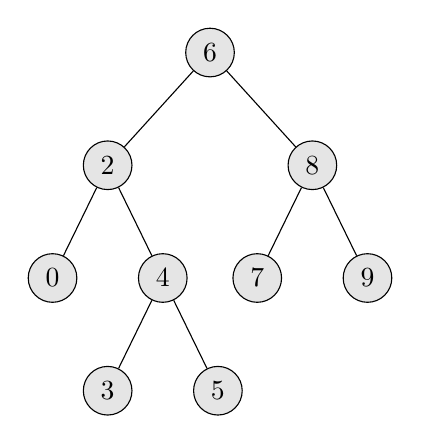
\begin{tikzpicture}
[mynode/.style={draw,circle,minimum size=5mm, fill=gray!20!}]
\node(){};
\node[mynode](1) {6};
\node[mynode](2)[below=8mm of 1, xshift=-13mm] {2};
\node[mynode](3)[below=8mm of 1, xshift=13mm] {8};
\node[mynode](4)[below=8mm of 2, xshift=-7mm] {0};
\node[mynode](5)[below=8mm of 2, xshift=7mm] {4};
\node[mynode](6)[below=8mm of 3, xshift=-7mm] {7};
\node[mynode](7)[below=8mm of 3, xshift=7mm] {9};
\node[mynode](8)[below=8mm of 5, xshift=-7mm] {3};
\node[mynode](9)[below=8mm of 5, xshift=7mm] {5};
\draw (1) -- (2);
\draw (1) -- (3);
\draw (2) -- (4);
\draw (2) -- (5);
\draw (3) -- (6);
\draw (3) -- (7);
\draw (5) -- (8);
\draw (5) -- (9);
\end{tikzpicture}
\end{figure}
$p = 2$, $q = 8$
\\
\textbf{Output}: 6
\\
\textbf{Explanation}: 
\\
The LCA of nodes 2 and 8 is 6.
\end{flushleft}

\paragraph{Example 2:}

\begin{flushleft}
\textbf{Input}:
\begin{figure}[H]
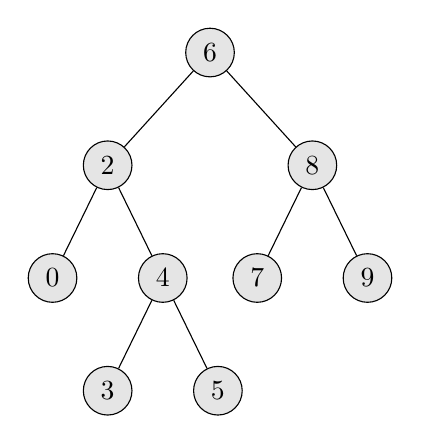
\begin{tikzpicture}
[mynode/.style={draw,circle,minimum size=5mm, fill=gray!20!}]
\node(){};
\node[mynode](1) {6};
\node[mynode](2)[below=8mm of 1, xshift=-13mm] {2};
\node[mynode](3)[below=8mm of 1, xshift=13mm] {8};
\node[mynode](4)[below=8mm of 2, xshift=-7mm] {0};
\node[mynode](5)[below=8mm of 2, xshift=7mm] {4};
\node[mynode](6)[below=8mm of 3, xshift=-7mm] {7};
\node[mynode](7)[below=8mm of 3, xshift=7mm] {9};
\node[mynode](8)[below=8mm of 5, xshift=-7mm] {3};
\node[mynode](9)[below=8mm of 5, xshift=7mm] {5};
\draw (1) -- (2);
\draw (1) -- (3);
\draw (2) -- (4);
\draw (2) -- (5);
\draw (3) -- (6);
\draw (3) -- (7);
\draw (5) -- (8);
\draw (5) -- (9);
\end{tikzpicture}
\end{figure}
$p = 2$, $q = 4$
\\
\textbf{Output}: 2
\\
\textbf{Explanation}: 
\\
The LCA of nodes 2 and 4 is 2, since a node can be a descendant of itself according to the LCA definition.
\end{flushleft}

\paragraph{Note:}

\begin{itemize}
\item All of the nodes' values will be unique.
\item $p$ and $q$ are different and both values will exist in the \texttt{BST}.
\end{itemize}
\subsection{BST Search}

借助\texttt{BST}的特性,由于题目中说明了每个节点的value都是unique的,所以
\begin{itemize}
\item 当根节点的value比$p$和$q$的value都大时,说明$p$和$q$的\texttt{LCA}在左子树,因此递归到左子树寻找。
\item 当根节点的value比$p$和$q$的value都大小时,说明$p$和$q$的\texttt{LCA}在右子树,因此递归到右子树寻找。
\item 否则,根节点的value处于$p$和$q$的value中间,因此根节点就是$p$和$q$的\texttt{LCA}。
\end{itemize}

\setcounter{lstlisting}{0}
\begin{lstlisting}[style=customc, caption={BST Properties}]
TreeNode* LCA( TreeNode* root, TreeNode* p, TreeNode* q )
{
    if( !root )
    {
        return root;
    }

    if( ( root->val > p->val ) && ( root->val > q->val ) )
    {
        //LCA in left subtree
        return LCA( root->left, p, q );
    }

    if( ( root->val < p->val ) && ( root->val < q->val ) )
    {
        //LCA in right subtree
        return LCA( root->right, p, q );
    }

    return root;
}

\end{lstlisting}
\section{236 --- Lowest Common Ancestor of a Binary Tree}
Given a binary tree, find the lowest common ancestor (\texttt{LCA}) of two given nodes in the tree.
\par
According to the definition of \texttt{LCA} on \textbf{Wikipedia}: \textit{The lowest common ancestor is defined between two nodes $p$ and $q$ as the lowest node in $T$ that has both $p$ and $q$ as descendants (where we allow \textbf{a node to be a descendant of itself}).}

\paragraph{Example 1:}

\begin{flushleft}
\textbf{Input}: 
\begin{figure}[H]
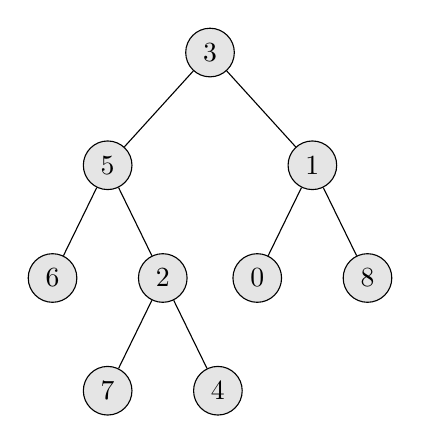
\begin{tikzpicture}
[mynode/.style={draw,circle,minimum size=5mm, fill=gray!20!}]
\node(){};
\node[mynode](1) {3};
\node[mynode](2)[below=8mm of 1, xshift=-13mm] {5};
\node[mynode](3)[below=8mm of 1, xshift=13mm] {1};
\node[mynode](4)[below=8mm of 2, xshift=-7mm] {6};
\node[mynode](5)[below=8mm of 2, xshift=7mm] {2};
\node[mynode](6)[below=8mm of 3, xshift=-7mm] {0};
\node[mynode](7)[below=8mm of 3, xshift=7mm] {8};
\node[mynode](8)[below=8mm of 5, xshift=-7mm] {7};
\node[mynode](9)[below=8mm of 5, xshift=7mm] {4};
\draw (1) -- (2);
\draw (1) -- (3);
\draw (2) -- (4);
\draw (2) -- (5);
\draw (3) -- (6);
\draw (3) -- (7);
\draw (5) -- (8);
\draw (5) -- (9);
\end{tikzpicture}
\end{figure}
$p = 5$, $q = 1$
\\
\textbf{Output}: 6
\\
\textbf{Explanation}: 
\\
The LCA of nodes 5 and 1 is 3.
\end{flushleft}

\paragraph{Example 2:}

\begin{flushleft}
\textbf{Input}:
\begin{figure}[H]
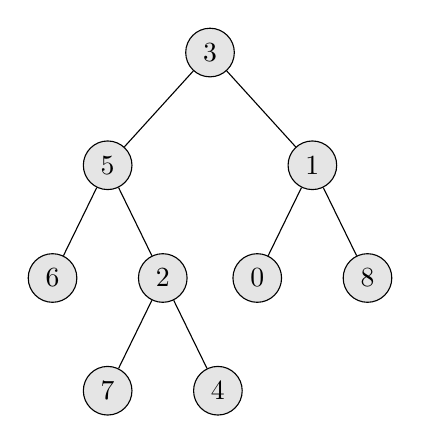
\begin{tikzpicture}
[mynode/.style={draw,circle,minimum size=5mm, fill=gray!20!}]
\node(){};
\node[mynode](1) {3};
\node[mynode](2)[below=8mm of 1, xshift=-13mm] {5};
\node[mynode](3)[below=8mm of 1, xshift=13mm] {1};
\node[mynode](4)[below=8mm of 2, xshift=-7mm] {6};
\node[mynode](5)[below=8mm of 2, xshift=7mm] {2};
\node[mynode](6)[below=8mm of 3, xshift=-7mm] {0};
\node[mynode](7)[below=8mm of 3, xshift=7mm] {8};
\node[mynode](8)[below=8mm of 5, xshift=-7mm] {7};
\node[mynode](9)[below=8mm of 5, xshift=7mm] {4};
\draw (1) -- (2);
\draw (1) -- (3);
\draw (2) -- (4);
\draw (2) -- (5);
\draw (3) -- (6);
\draw (3) -- (7);
\draw (5) -- (8);
\draw (5) -- (9);
\end{tikzpicture}
\end{figure}
$p = 5$, $q = 4$
\\
\textbf{Output}: 5
\\
\textbf{Explanation}: 
\\
The LCA of nodes 5 and 4 is 5, since a node can be a descendant of itself according to the LCA definition.
\end{flushleft}

\paragraph{Note:}

\begin{itemize}
\item All of the nodes' values will be unique.
\item $p$ and $q$ are different and both values will exist in the binary tree.
\end{itemize}
\subsection{Recursion}
这道题和235不同,这里只是一般的bianry tree。
\begin{itemize}
\item 按照深度优先的方式遍历tree。
\item 当遇到$p$或者$q$时,返回一些boolean flags。这些flags会帮助确定是否在某个path上找到了$p$或者$q$。
\item \texttt{LCA}则是其对其左右子树进行递归处理都能够返回\texttt{true}的那个节点。
\item 由于\texttt{LCA}也可能是$p$或者$q$中的一个,这种情况下只会有一个子树返回\texttt{true}
\end{itemize}
算法过程如下
\begin{itemize}
\item 从root开始遍历tree。
\item 如果current node本身就是$p$或者是$q$,将一个变量$x$设为\texttt{true},然后继续在左右子树中寻找另外一个节点。
\item 如果遍历左子树的结果$l$或者遍历右子树$r$是\texttt{true},表明$p$和$q$中的一个被找到了。
\item 在遍历过程中,任何时候发现$l$, $r$和$x$这三个变量中有两个为\texttt{true}了,表明已经找到了$p$和$q$的\texttt{LCA}。
\item 具体实现时,用$l$, $r$和$x$都设为\texttt{int}。这样可以通过判断这三个的和来判定是否有两个为\texttt{true}。
\end{itemize}
\setcounter{lstlisting}{0}
\begin{lstlisting}[style=customc, caption={Recursion}]
TreeNode* LCA( TreeNode* root, TreeNode* p, TreeNode* q )
{
    TreeNode* ans;
    dfs( root, p, q, ans );

    return ans;
}

bool dfs( TreeNode* node, TreeNode* p, TreeNode* q, TreeNode*& lca )
{
    if( !node )
    {
        return false;
    }

    int x = 0;

    if( ( node == p ) || ( node == q ) )
    {
        //one of p and q is found
        x = 1;
    }

    int l = 0;
    if( dfs( node->left, p, q, lca ) )
    {
        //Found p and/or q in left tree
        l = 1;
    }

    int r = 0;
    if( dfs( node->right, p, q, lca ) )
    {
        //Found p and/or q in right tree
        r = 1;
    }

    if( l + r + x >= 2 )
    {
        //LCA is found
        lca = node;
    }

    return ( l + r + x ) > 0; //at least find one of p and q
}
\end{lstlisting}
\subsection{Another Recursion}
\begin{CJK*}{UTF8}{gbsn}
在binary tree中搜索$p$和$q$,然后从遍历路径中找到最后一个相同的节点即为\texttt{LCA}。边界情况很简单: 首先看当前结点是否为\texttt{null},若为\texttt{null}则直接返回\texttt{null},若为$p$或$q$中的任意一个,直接返回当前结点
\par
如果当前结点不等于$p$或$q$,$p$和$q$要么分别位于左右子树中,要么同时位于左子树,或者同时位于右子树
\begin{itemize}
\item 若$p$和$q$分别位于左右子树中,那么对左右子结点进行recursion,会分别返回$p$和$q$结点的位置,而当前结点正好就是$p$和$q$的最小共同父结点,直接返回当前结点即可,这就是题目中的例子1的情况。
\item 若$p$和$q$同时位于左子树,这时候调用递归函数处理right subtree会返回\texttt{null}, 而处理left subtree有两种情况,
\begin{enumerate}
\item 函数返回的是$p$和$q$中靠近根节点的那个节点,这时候返回这个节点。这就是题目中的例子2的情况。
\item 函数返回的是$p$和$q$的\texttt{LCA},就是说当前结点的左子树中的某个结点才是$p$和$q$的\texttt{LCA},也直接返回这个结果。
\end{enumerate}
\item 若$p$和$q$同时位于右子树,和上述左子树情形类似。
\end{itemize}
\end{CJK*}
\begin{lstlisting}[style=customc, caption={Recursion Based On Left And Right Subtree}]
TreeNode* LCA( TreeNode* root, TreeNode* p, TreeNode* q )
{
    if( !root || root == p || root == q )
    {
        return root;
    }

    //process left subtree
    auto l_node = LCA( root->left, p, q );
    //process right subtree
    auto r_node = LCA( root->right, p, q );

    //found the two nodes in left and right subtree respectively
    //LCA is found
    if( l_node && r_node )
    {
        return root;
    }

    //p and q only in left subtree
    if( l_node )
    {
        return l_node;
    }

    //p and q only in right subtree
    return r_node;
}
\end{lstlisting}
\subsection{Iterative using parent pointers}
\begin{CJK*}{UTF8}{gbsn}
这种方法则需要借助queue和hash map来寻找最接近$p$和$q$的common ancestor。
\par
算法步骤如下
\begin{enumerate}
\item 从根节点开始遍历tree。由于是iterative traverse,所以需要借助queue。
\item 将当前节点的parent node保存在一个hash map $M$中直到找到$p$和$q$。
\item 一旦找到$p$和$q$,将$p$的所有ancestors从$M$中加入到一个hash set $S$中。
\item 然后在$M$中遍历$q$所有的ancestors。如果当前遇到的ancestor可以在$S$中找到,这就是$p$和$q$的\texttt{LCA}。
\end{enumerate}
\end{CJK*}
\begin{lstlisting}[style=customc, caption={Iterative Searching}]
TreeNode* LCA( TreeNode* root, TreeNode* p, TreeNode* q )
{

    queue<TreeNode*> qt;
    unordered_map<TreeNode*, TreeNode*> m;

    qt.push( root );
    m.emplace( root, nullptr ); //root's parent is empty

    //iterative traverse the tree using the queue
    while( !qt.empty() )
    {
        auto it_p = m.find( p );
        auto it_q = m.find( q );

        if( ( it_p != m.end() ) && ( it_q != m.end() ) )
        {
            //p and q both are found
            break;
        }

        auto t = qt.front();
        qt.pop();

        if( t->left )
        {
            m.emplace( t->left, t );
            qt.emplace( t->left );
        }

        if( t->right )
        {
            m.emplace( t->right, t );
            qt.emplace( t->right );
        }
    }

    unordered_set<TreeNode*> A;

    // add all p's ancestors into the hash set A
    auto t = p;
    while( t )
    {
        A.insert( t );
        t = m[t];
    }

    // find the first ancestor of q that
    // can be found in A
    t = q;
    while( t )
    {
        auto it = ancestors.find( t );

        if( it != ancestors.end() )
        {
            return *it;
        }

        t = m[t];
    }

    // cannot find LCA
    return nullptr;
}
\end{lstlisting}

\section{239 --- Sliding Window Maximum}
Given an array $A$, there is a sliding window of size $k$ which is moving from the very left of the array to the very right. You can only see the $k$ numbers in the window. Each time the sliding window moves right by one position. Return the \texttt{max} sliding window.

\paragraph{Example:}
\begin{flushleft}
\textbf{Input}: \fcj{A = [1,3,-1,-3,5,3,6,7]}, and $k = 3$
\\
\textbf{Output}: \fcj{[3,3,5,5,6,7]}
\\
\textbf{Explanation:} 
\begin{itemize}
\item $[1,\;  3,\;  -1],\; -3,\;  5,\;  3,\;  6,\;  7 \Longrightarrow       3$
\item $1,\; [3,\;  -1,\;  -3,\;] 5,\;  3,\;  6,\;  7 \Longrightarrow       3$
\item $1,\;  3,\; [-1,\;  -3,\;  5],\; 3,\;  6,\;  7 \Longrightarrow 5$
\item $1,\; 3,\; -1,\;[-3,\; 5,\; 3],\; 6,\; 7 \Longrightarrow 5$
\item $1,\;  3,\;  -1,\;  -3,\; [5,\;  3,\;  6],\; 7 \Longrightarrow       6$
\item $1,\; 3,\; -1,\;  -3,\;  5,\; [3,\;  6,\;  7]  \Longrightarrow  7$
\end{itemize}
\end{flushleft}
\paragraph{Note:}
\begin{itemize}
\item You may assume $k$ is always valid, $1 \leq k \leq$ input array's size for non-empty array.
\end{itemize}
\paragraph{Follow up:}
\begin{itemize}
\item Could you solve it in linear time?
\end{itemize}
\subsection{Double-End Queue}
所有的固定长度滑动窗口问题都有可以用double-end queue来作为基础的数据结构。
\begin{itemize}
\item 遍历数组$A$。用一个double-end queue $q$来存放访问的index
。
\item 在当前index $i$,如果$q$的\texttt{front}刚好等于$i-k$,那么就将\texttt{front}从$q$中去除。因为这时候滑动窗口已经不再包含距离大于$k$的元素了。
\item 然后进入一个循环比较$q$的\texttt{back}是否小于或者等于当前数字,如果小于或者等于,一直将\texttt{back}从$q$中移除。
\item 然后将$i$加入到$q$的后面。
\item 如果$i\geq k$,这时候就要输出最大值了,而最大值就是$q$的front。
\end{itemize}

\setcounter{lstlisting}{0}
\begin{lstlisting}[style=customc, caption={Deque}]
vector<int> maxSlidingWindow( vector<int>& nums, int k )
{
    int L = static_cast<int>( nums.size() );
    deque<int> q;
    vector<int> m;
    m.reserve( L - k + 1 );
    for( int i = 0; i < L; ++i )
    {
        //pop out index outside sliding window
        if( !q.empty() && ( q.front() == i - k ) )
        {
            q.pop_front();
        }
        //pop out back index where numbers are no larger than
        //current number
        while( !q.empty() && ( nums[q.back()] <= nums[i] ) )
        {
            q.pop_back();
        }
        //add current index to q's back end
        q.push_back( i );
        // need to output maximum of sliding window
        // from k-1 to L-1
        if( i >= k - 1 )
        {
            m.push_back( nums[q.front()] );
        }
    }
    return m;
}
\end{lstlisting}
\section{287 --- Find the Duplicate Number}
Given an array $A$ containing $n + 1$ integers where each integer is between 1 and $n$ (inclusive), prove that at least one duplicate number must exist. Assume that there is only one duplicate number, find the duplicate one.

\paragraph{Example 1:}
\begin{flushleft}
\textbf{Input}: $[1,3,4,2,2]$
\\
\textbf{Output}: 2
\end{flushleft}

\paragraph{Example 2:}
\begin{flushleft}
\textbf{Input}: $[3,1,3,4,2]$
\\
\textbf{Output}: 3
\end{flushleft}

\paragraph{Note:}
\begin{itemize}
\item You must not modify the array (assume the array is read only).
\item You must use only constant, $O(1)$ extra space.
\item Your runtime complexity should be less than $O(n^2)$.
\item There is only one duplicate number in the array, but it could be repeated more than once.
\end{itemize}
\subsection{Detect Cycle And Find The Cycle Start}
\begin{itemize}
\item 与检测链表是否有cycle并找到cycle的起始点类似。
\item 由于存在重复元素,并且$A$中每个值的大小都是1到$n$,而长度又是$n+1$,因此如果将$A[i]$看作index,那么根据$A[i]$的值访问下个元素$A[A[i]]$到最后就会形成cycle。
\item 另外由于0不属于1到$n$,因此$A[0]$肯定不在cycle内,这就相当于有cycle的链表里,链表的头指针不在cycle中。
\item 借用链表中的快慢指针,这里用两个index$x$和$y$分别代表快慢两个index,其中$x\gets A[A[x]]$ 而$y\gets A[y]$。如果遇到相等,就终止循环,
\item 然后$x$和$y$分别从0和刚才循环中断的地方开始按照$i\gets A[i]$的方式前进,直到相等,这个相等的位置处即为重复的number。
\end{itemize}
\setcounter{algorithm}{0}
\begin{algorithm}[H]
\caption{Detect Cycle And Find Cycle Start}
\begin{algorithmic}[1]
\Procedure{FindDuplicate}{$A$}
\State $\ast$ 初始化两个index $x$和$y$为0
\State $\ast$ 检测Cycle,找到快慢两个index的相遇点
\Repeat
\State $x\gets A[A[x]]$
\State $y\gets A[y]$
\Until{$x=y$}
\State $\ast$ 寻找Cycle的起始点
\State $z:=0$ \Comment 找起始点也需要两个index,其中一个是0,另外一个就是刚才找到的相遇点
\Repeat
\State $x\gets A[x]$
\State $z\gets A[z]$
\Until{$x=z$}
\State \Return $x$
\EndProcedure
\end{algorithmic}
\end{algorithm}
\setcounter{lstlisting}{0}
\begin{lstlisting}[style=customc, caption={Detect Cycle And Find Cycle Start}]
int findDuplicate( vector<int>& nums )
{
    //x is the fast index
    //y is the slow index
    int x = 0;
    int y = 0;

    //detect cycle and
    //find the meet point of x and y
    do
    {
        x = nums[nums[x]];
        y = nums[y];
    }
    while( x != y );

    //find the start of the cycle
    //one index will start from 0
    //since nums[0] is not inside cycle
    int z = 0;

    while( x != z )
    {
        x = nums[x];
        z = nums[z];
    }

    return x;
}
\end{lstlisting}
\subsection{Binary Search}
\paragraph{Why Binary Search Can Work}
\begin{enumerate}
\item 由于所有数字的范围都是$1$到$n$,那么如果$A$中没有重复数字,那么对于一个数$x$,在$A$小于或者等于$x$的数字个数就为$x$个。
\item 但由于$A$中有重复的数字,假设这个数字是$m$,那么$A$中小于或者等于这个重复数字$m$的至少有$m+1$个。由于$A$的长度为$n+1$,因此对$A$中其他数,小于或者等于这个数的个数都不会大于这个数本身。
\item 因此binary search是要在$1$到$n$这$n$个数中找到第一个数$\alpha$使得在$A$中小于等于$\alpha$的数的个数$z$要大于$\alpha$。典型的\textbf{rightmost} binary search。
\item 注意binary search不是作用于数组$A$。
\end{enumerate}
\paragraph{Algorithm Steps}
\begin{itemize}
\item 初始化左右两端的index $l$和$r$分别为1和$n$。
\item 得到当前的middle value $x=(l+r)/2$,遍历$A$,得到小于等于$x$的数的count $z$,
\begin{enumerate}
\item 如果$z\leq x$,$l\gets x+1$
\item 如果$z > x$,$r\gets x$
\item 循环结束后 $l$就是那个duplicate number。
\end{enumerate}
\end{itemize}
\begin{algorithm}[H]
\caption{Binary Search}
\begin{algorithmic}[1]
\Procedure{FindDuplicate}{$A,L$}
\State $l:=1$, $r:=L-1$ \Comment Binary Search on $[1,n]$ not on $A$ and $L=n+1$
\State $\ast$ Rightmost Binary Search
\While{$l < r$}
\State $x:=(l+r)/2$ \Comment Mid-point
\State $z:=0$
\For{Each number $t$ in $A$}
\If{$t \leq x$}
\State $z\gets z+1$
\EndIf
\EndFor
\If{$z\leq x$}
\State $l\gets x+1$
\Else
\State $r\gets x$
\EndIf
\EndWhile
\State \Return $l$
\EndProcedure
\end{algorithmic}
\end{algorithm}
\begin{lstlisting}[style=customc, caption={Binary Search}]
int findDuplicate( vector<int>& nums )
{
    int l = 1;
    //r=n
    int r = static_cast<int>( nums.size() ) - 1;

    //binary search on $[1...n]$
    //not on nums
    while( l < r )
    {
        int x = ( l + r ) / 2;

        int count = 0;
        for( int n : nums )
        {
            if( n <= x )
            {
                ++count;
            }
        }

        if( count <= x )
        {
            l = x + 1;
        }
        else
        {
            r = x;
        }
    }

    return l;
}
\end{lstlisting}
\subsection{Bit Manipulation}
\begin{itemize}
\item 在总共32个bit位上,分别统计出1到$n$上在每个比特位上的1的个数,记为$x$
\item 同样的在总共32个bit位上,分别统计出$A$中所有数字在每个比特位上的1的个数,记为$y$。
\item 如果在某个bit位上,$y>x$,表明该位上肯定有重复数字的贡献,因此将结果中的对应的bit位也设为1。
\item 这样32个bit位上设置好相应的bit 1后,就能得到那个重复数字。
\end{itemize}
\setcounter{lstlisting}{0}
\begin{lstlisting}[style=customc, caption={Bit Manipulation}]
int findDuplicate( vector<int>& nums )
{
    int mask = 1;

    int L = static_cast<int>( nums.size() );

    int ans = 0;

    for( int i = 0; i < 32; ++i )
    {
        //in fact, x counts for [0...n]
        //but 0 has no any effect
        mask = 1 << i;

        int x = 0;
        int y = 0;

        for( int i = 0; i < L; ++i )
        {
            if( i & mask )
            {
                ++x;
            }

            if( nums[i] & mask )
            {
                ++y;
            }
        }

        if( y > x )
        {
            ans |= mask;
        }
    }

    return ans;
}
\end{lstlisting}
\section{480 --- Sliding Window Median}
Median is the middle value in an ordered integer list. If the size of the list is even, there is no middle value. So the median is the mean of the two middle value.

Given an array $A$, there is a sliding window of size $k$ which is moving from the very left of the array to the very right. You can only see the $k$ numbers in the window. Each time the sliding window moves right by one position. Your job is to output the median array for each window in the original array.

\paragraph{Example:}

\begin{flushleft}
\textbf{Input}:  $A = [1,3,-1,-3,5,3,6,7]$, $k=3$

\textbf{Output}: $[1,-1,-1,3,5,6]$

\textbf{Explanation}

\begin{table}[H]
\begin{tabular}{cc}
Window Position & Median \\
\hline
$[1 \; 3 \; -1]$  $-3\   5\   3 \  6 \ 7$ & $1$ \\
1 $[3  -1  -3]$ 5  3  6  7 & $-1$ \\
1  3 [$-1$  $-3$  5] 3  6  7 &       $-1$ \\
1  3  $-1$ [$-3 $ 5  3] 6  7   &    3 \\
1  3  $-1$  $-3$ [5  3  6] 7   &    5 \\ 
1  3  $-1$  $-3$  5 [3  6  7]      6
\end{tabular}
\end{table}

\end{flushleft}

\paragraph{Note: }
\begin{itemize}
\item You may assume $k$ is always valid, ie: $k$ is always smaller than input array's size for non-empty array.
\end{itemize}


\subsection{Median For Stream Values}

\setcounter{lstlisting}{0}
\begin{lstlisting}[style=customc, caption={Using Two Heaps}]
class Solution
{
public:
    vector<double> medianSlidingWindow( vector<int>& nums, int k )
    {
        auto L = static_cast<int>( nums.size() );

        //put first k elements into lower half
        for( int i = 0; i < k; ++i )
        {
            pq_low.push( nums[i] );
        }

        //put k/2 upper elements from pq_low
        //to pq_up

        for( int i = 0; i < k / 2; ++i )
        {
            pq_up.push( pq_low.top() );
            pq_low.pop();
        }

        auto get_median = [this]( int k ) -> double
        {
            if( k & 1 )
            {
                return this->pq_low.top();
            }

            auto x = static_cast<double>( this->pq_up.top() );
            auto y = static_cast<double>( this->pq_low.top() );

            return ( x + y ) * .5;
        };

        vector<double> ans;


        for( int i = k; i < L; ++i )
        {
            if( pq_low.empty() )
            {
                //this cannot happen
                break;
            }

            ans.emplace_back( get_median( k ) );

            int left = nums[i - k]; //the element to be removed
            int n = nums[i];

            //changes of difference between
            //the number elements of lower half and
            //upper half
            int delta_diff = 0;

            //remove left from two queues
            remove( left, delta_diff );

            //insert new elements
            insert( n, delta_diff );

            //rebalance two queues
            //make sure difference between
            //the number elements of lower half and
            //upper half is same as before
            reblance( delta_diff );

            //clean up the two queues
            //remove those elements that should be removed
            //but still in each queue's top. These elements
            //may effect the computation of median value
            clean();
        }

        //we have not add the last window's median value
        ans.emplace_back( get_median( k ) );

        return ans;
    }

private:

    void remove( int n, int& delta )
    {
        bool is_top = false;

        if( n <= pq_low.top() )
        {
            //n is inside lower half
            //the delta of difference decrements
            //since we will remove n from lower half
            --delta;
            if( pq_low.top() == n )
            {
                is_top = true;
                pq_low.pop();
            }
        }
        else
        {
            //n is inside upper half
            //the delta of difference increments
            //since we will remove n from upper half
            ++delta;

            if( pq_up.top() == n )
            {
                is_top = true;
                pq_up.pop();
            }
        }

        if( !is_top )
        {
            //put it into the map
            //records the elements
            //should be removed

            //we cannot remove them right now
            //because they may decide the
            //median value
            auto it = m_remove.find( n );
            if( it == m_remove.end() )
            {
                m_remove.emplace( n, 1 );
            }
            else
            {
                ++it->second;
            }
        }

    }

    void insert( int n, int& delta )
    {
        if( !pq_low.empty() && ( n <= pq_low.top() ) )
        {
            //n belongs to lower half
            //increments the delta of difference
            ++delta;

            pq_low.push( n );
        }
        else
        {
            //n may belong to upper half
            --delta;
            pq_up.push( n );
        }
    }

    void reblance( int delta )
    {
        if( delta < 0 )
        {
            //lower half have fewer items
            //add smallest item from upper half
            pq_low.push( pq_up.top() );
            pq_up.pop();
        }
        else if( delta > 0 )
        {
            //upper half have fewer items
            //add largest item from lower half
            pq_up.push( pq_low.top() );
            pq_low.pop();
        }
    }

    void clean()
    {
        while( !pq_low.empty() )
        {
            auto it = m_remove.find( pq_low.top() );
            if( it == m_remove.end() )
            {
                break;
            }

            //since the element should be removed
            //is at the top of queue
            //we must remove it, otherwise, the median
            //maybe wrong
            pq_low.pop();
            it->second -= 1;
            if( it->second == 0 )
            {
                //the element has been removed
                m_remove.erase( it );
            }
        }

        while( !pq_up.empty() )
        {
            auto it = m_remove.find( pq_up.top() );
            if( it == m_remove.end() )
            {
                break;
            }

            //since the element should be removed
            //is at the top of queue
            //we must remove it, otherwise, the median
            //maybe wrong
            pq_up.pop();
            it->second -= 1;
            if( it->second == 0 )
            {
                //the element has been removed
                m_remove.erase( it );
            }
        }
    }

private:

    //lower half
    priority_queue<int> pq_low;

    //upper half
    priority_queue<int, vector<int>, greater<int>> pq_up;

    //the hash map that contains the
    //elements would be removed
    //but still kept in the two queues
    unordered_map<int, int> m_remove;

};
\end{lstlisting}
\section{1114 --- Print in Order}
Suppose we have a class:

\begin{lstlisting}[style=customc]
public class Foo {
  public void one() { print(one); }
  public void two() { print(two); }
  public void three() { print(three); }
}
\end{lstlisting}

The same instance of \texttt{Foo} will be passed to three different threads. Thread $A$ will call \texttt{one}, thread $B$ will call \texttt{two}, and thread $C$ will call \texttt{three}. Design a mechanism and modify the program to ensure that \texttt{two} is executed after \texttt{one}, and \texttt{three} is executed after \texttt{two}.

 

\paragraph{Example 1:}

\begin{flushleft}
\textbf{Input}: $[1,2,3]$

\textbf{Output}: \texttt{onetwothree}

\textbf{Explanation}: 

There are three threads being fired asynchronously. 

The input $[1,2,3]$ means thread $A$ calls \texttt{one}(), thread $B$ calls \texttt{two}(), and thread $C$ calls \texttt{three}(). 

\texttt{onetwothree} is the correct output.
\end{flushleft}


\paragraph{Example 2:}

\begin{flushleft}
\textbf{Input}: $[1,3,2]$

\textbf{Output}: \texttt{onetwothree}

\textbf{Explanation}: 

The input $[1,3,2]$ means thread $A$ calls \texttt{one}(), thread $B$ calls \texttt{three}(), and thread $C$ calls \texttt{two}(). \texttt{onetwothree} is the correct output.
\end{flushleft}
 

\paragraph{Note:}

\begin{itemize}
\item We do not know how the threads will be scheduled in the operating system, even though the numbers in the input seems to imply the ordering. The input format you see is mainly to ensure our tests' comprehensiveness.
\end{itemize}

\subsection{Condition Variable}
In C++ 11 and later, The \texttt{condition\_variable} class is a synchronization primitive that can be used to block a thread, or multiple threads at the same time, until another thread both modifies a shared variable (the condition), and notifies the \texttt{condition\_variable}.

\setcounter{lstlisting}{0}
\begin{lstlisting}[style=customc, caption={Condition Variable}]
class Foo
{
public:
    Foo()
    {
        m_flag1 = false;
        m_flag2 = false;
    }

    void first( function<void()> printFirst )
    {
        // printFirst() outputs "first". Do not change or remove this line.
        printFirst();
        m_flag1 = true;
        m_cv1.notify_one();
    }

    void second( function<void()> printSecond )
    {
        // printSecond() outputs "second". Do not change or remove this line.
        unique_lock<mutex> lk( m_mtx );
        m_cv1.wait( lk, [this] {return m_flag1;} ); //when m_flag1 is true, m_cv1 will stop waiting
        printSecond();
        m_flag2 = true;
        m_cv2.notify_one();
    }

    void third( function<void()> printThird )
    {

        unique_lock<mutex> lk( m_mtx );
        m_cv2.wait( lk, [this] {return m_flag2;} ); //when m_flag2 is true, m_cv1 will stop waiting
        // printThird() outputs "third". Do not change or remove this line.
        printThird();
    }

    mutex m_mtx;
    condition_variable m_cv1;
    condition_variable m_cv2;

    bool m_flag1;
    bool m_flag2;
};
\end{lstlisting}
\section{1115 --- Print FooBar Alternately}
Suppose you are given the following code:

\begin{lstlisting}[style=customc]
class FooBar {
  public void foo() {
    for (int i = 0; i < n; i++) {
      print(foo);
    }
  }

  public void bar() {
    for (int i = 0; i < n; i++) {
      print(bar);
    }
  }
}
\end{lstlisting}

The same instance of \texttt{FooBar} will be passed to two different threads. Thread A will call \texttt{foo} while thread B will call \texttt{bar}. Modify the given program to output \texttt{foobar} $n$ times.

\paragraph{Example 1:}

\begin{flushleft}
\textbf{Input}: $ n = 1 $

\textbf{Output}: \texttt{foobar}

\textbf{Explanation}: There are two threads being fired asynchronously. One of them calls \texttt{foo}, while the other calls \texttt{bar}. \texttt{foobar} is being output 1 time.

\end{flushleft}

\paragraph{Example 2:}

\begin{flushleft}
\textbf{Input}: $ n = 2 $

\textbf{Output}: \texttt{foobarfoobar}

\textbf{Explanation}: \texttt{foobar} is being output 2 times.
\end{flushleft}

\subsection{Condition Variable}

\setcounter{lstlisting}{0}
\begin{lstlisting}[style=customc, caption={Condition Variable}]
class FooBar {
private:
    int n;
    
    mutex m_mtx;
    condition_variable m_cv;
    
    bool m_flag;

public:
    FooBar(int n) {
        this->n = n;
        m_flag = true; //show foo
    }

    void foo(function<void()> printFoo) {
        
        unique_lock<mutex> lk(m_mtx);
        for (int i = 0; i < n; i++) {
            m_cv.wait(lk, [this]{return m_flag;});
        	// printFoo() outputs "foo". Do not change or remove this line.
        	printFoo();
            
            m_flag = false;
            lk.unlock();
            m_cv.notify_one();
            lk.lock();
        }
    }

    void bar(function<void()> printBar) {
         unique_lock<mutex> lk(m_mtx);
        for (int i = 0; i < n; i++) {
            m_cv.wait(lk, [this]{return !m_flag;});
        	// printBar() outputs "bar". Do not change or remove this line.
        	printBar();
            
            m_flag = true;
            
            lk.unlock();
            m_cv.notify_one();
            lk.lock();
        }
    }
};
\end{lstlisting}

\begin{lstlisting}[style=customc, caption={1117}]
class H2O
{
    mutex m;
    condition_variable cv;
    int c = 1;
public:
    H2O()
    {
    }
    void hydrogen( function<void()> releaseHydrogen )
    {
        unique_lock<mutex> lk( m );
        cv.wait( lk, [this] {return ( c % 3 != 0 );} );
        // releaseHydrogen() outputs "H". Do not change or remove this line.
        releaseHydrogen();
        ++c;
        if( !( c % 3 ) )
        {
            lk.unlock();
            cv.notify_all();
        }
    }
    void oxygen( function<void()> releaseOxygen )
    {
        unique_lock<mutex> lk( m );
        cv.wait( lk, [this] {return ( c % 3 == 0 );} );
        // releaseOxygen() outputs "O". Do not change or remove this line.
        releaseOxygen();
        ++c;
        lk.unlock();
        cv.notify_one();
    }
};
\end{lstlisting}
\end{document}